% !TeX root = ../thesis.tex
% ------------------------------------------------
%
%論文內容次序:
% 1.考試合格證明
% 2.中英文摘要(論文以中文撰寫者須附英文延伸摘要)
% 3.誌謝
% 4.目錄
% 5.表目錄
% 6.圖目錄
% 7.符號
% 8.主文
% 9.參考文獻
% 10.附錄
%
% 註: 參考文獻書寫注意事項:
% (1).
%    文學院之中文文獻依分類及年代順序排列。
%    其他學院所之文獻依英文姓氏第一個字母
%    (或中文姓氏第一個字筆劃)及年代順序排列。
%
% (2).
%    期刊文獻之書寫依序為:
%        姓名、文章名稱、期刊名、卷別、期別、頁別、年代。
%
% (3).
%    書寫之文獻依序為:
%        姓名、書名、出版商名、出版地、頁別、年代。
%
% ------------------------------------------------

% 封面內頁 Inner Cover
%
% 封面: 顯示所有封面內容, 但沒有學校Logo)
%     主要用在印刷版, 如精裝版 或 平裝版
%     (使用cover.tex來產生)
%
% 內頁: 顯示所有封面內容, 但有學校Logo
%     主要用在電子版 + 印刷版
%
% 只要是印刷版, 不論是精裝版或平裝版, 都是 封面 (殼/皮) + 內頁.
% 只有在電子版時, 第一頁就是封面內頁.

\DisplayInnerCover

% ------------------------------------------------

% 學位考試論文證明書
\DisplayOral

% ------------------------------------------------

% 摘要 Abstract
% 除了外籍生, 本地生和僑生都是要編寫中文和英文摘要
% 論文以中文撰寫須以英文補寫 800 至 1200 字數的英文延伸摘要 (Extended Abstract)
% 詳細可看附件的學校要求或看example中的英文延伸摘要

% !TeX root = ../../thesis.tex
% ------------------------------------------------
\StartAbstractChi
% ------------------------------------------------

除了外籍生, 本地生和僑生都是要編寫中文和英文摘要. 論文以中文撰寫須以英文補寫 800 至 1200 字數的英文延伸摘要 (Extended Abstract), 如需要的話請修改`./context/abstract/extended.tex'.

外籍生則可免填中文摘要, 而在上傳時網頁資訊需填上`NONE'.\\

% ------------------------------------------------
\EndAbstractChi
% ------------------------------------------------
             % 中文版
% !TeX root = ../../thesis.tex
% ------------------------------------------------
\StartAcknowledgments
% ------------------------------------------------

Thanks someone you want in here.

% ------------------------------------------------
\EndAcknowledgments
% ------------------------------------------------
             % 英文版
%% !TeX root = ../../thesis.tex
% ------------------------------------------------
\StartExtendedAbstract
% ------------------------------------------------

\ExtAbstractSummary{%
The summary is a short, informative abstract of no more than 250 words. References should not be cited. The summary should (1) state the scope and objectives of the research, (2) describe the methods used, (3) summarize the results, and (4) state the principal conclusions. Text of the summary should be 12 pt Times New Roman font, single-spaced and justified. A single line space should be left below the title `SUMMARY'. Leave a single line space above the key words listed below.
} % End of \ExtAbstractSummary{}

% ------------------------------------------------

\ExtAbstractChapter{INTRODUCTION}
The purpose of the introduction is to tell readers why they should want to read your thesis/ dissertation. This section should provide sufficient background information to allow readers to understand and evaluate the paper's results.

The introduction should (1) present the nature and scope of the problem, (2) review related literature, (3) describe the materials used and method(s) of the study, and (4) describe the main results of the study.

All text in the main body of the extended abstract should be 12 pt Times New Roman font, single-spaced and justified. Main headings are placed in the centre of the column, in capital letters using 12 pt Times New Roman Bold font. Subheadings are placed on the left margin of the column and are typed in 12 pt Times New Roman Bold font.

% ------------------------------------------------

\ExtAbstractChapter{MATERIALS AND METHODS}
There is flexibility as to the naming of the section (or sections) that provide information on the method(s) or theories employed. The methodology employed inthe work must be described in sufficient detail or with sufficient references so that the results could be duplicated.

Your materials should be organised carefully. Include all the data necessary to support your conclusions, but exclude redundant or unnecessary data.

% ------------------------------------------------

\ExtAbstractChapter{RESULTS AND DISCUSSION}
The results and discussion sections present your research findings and your analysis of those findings. The results of experiments can be presented as tables or figures.

% ------------------------------------------------

\ExtAbstractSection{Figures and Tables}
Figures may be integrated within the results section of the extended abstract, or they can be appended to the end of the written text. Figures should be black \& white. They should be no wider than the width of the A4 page.

Tables can be created within Word. As noted for figures above, if a table is to be placed within the text, it can be no wider than the width of the A4 page. Larger tables will need to be placed at the end of the abstract.

Figures and tables should be numbered according to the order they are referenced in the paper. Figures and tables should be referred to by their number in the text. When referring to figures and tables in the text, spell out and capitalize the word Figure or Table. All figures and tables must have captions.

% ------------------------------------------------

\ExtAbstractSection{Captions}
Captions should clearly explain the significance of the figure or table without reference to the text. Details in captions should not be restated in the text. Parameters in figure captions should be included and presented in words rather than symbols.

Captions should be placed directly above the relevant table and beneath the relevant figure. The caption should be typed in 12 pt Times New Roman Bold font. Spell out the word `Table' or `Figure' in full. An example table and a figure follow.

% ------------------------------------------------

\InsertTable
  [caption={Specifications of the engine}]
  {
    \begin{tabular}{llll}
    \hline
    Engine &  &  & OPEL Astra C16SE \\ \hline
    Displacement (cc) &  &  & 1598 \\
    Bore x stroke(mm x mm) &  &  & 79 x 81.5 \\
    Value mechanism &  &  & SOHC \\
    Number of valves &  &  & Intake 4, exhaust 4 \\
    Compression ratio &  &  & 9.8:1 \\
    Torque &  &  & 135/3400 Nm/rpm \\
    Power &  &  & 74/5800 kW/rpm \\
    Ignition sequence &  &  & 1-3-4-2 \\
    Spark plug &  &  & BPR6ES \\
    Fuel &  &  & 95 unleaded gasoline \\
    Cylinder arrangment &  &  & In-line 4 cylinders \\ \hline
    \end{tabular}
  } % End of  \InsertTable{}

% \InsertFigure
%   [scale=0.5,
%     caption={HC emission as a function of equivalence ratio}]
%   {./example/abstract/pic/extended-abstract-2.jpg}

% ------------------------------------------------

\ExtAbstractChapter{CONCLUSION}
This section should include (1) the main points of your paper and why they are significant, (2) any exceptions to, problems with, or limitations to your argument, (3) agreements or disagreements with previously published work, (4) theoretical and practical implications of the work, and (5) conclusions drawn.

% ------------------------------------------------
\EndExtendedAbstract
% ------------------------------------------------
        % 英文延伸摘要

% ------------------------------------------------

% 誌謝 Acknowledgments
% 誌謝正常應該只要寫一種版本就可,
% 提供2種以自行選擇所顯示的語言.
% 2種同時編寫都是可以的.

% !TeX root = ../../thesis.tex
% ------------------------------------------------
\StartAbstractChi
% ------------------------------------------------

除了外籍生, 本地生和僑生都是要編寫中文和英文摘要. 論文以中文撰寫須以英文補寫 800 至 1200 字數的英文延伸摘要 (Extended Abstract), 如需要的話請修改`./context/abstract/extended.tex'.

外籍生則可免填中文摘要, 而在上傳時網頁資訊需填上`NONE'.\\

% ------------------------------------------------
\EndAbstractChi
% ------------------------------------------------
             % 中文版
% % !TeX root = ../../thesis.tex
% ------------------------------------------------
\StartAcknowledgments
% ------------------------------------------------

Thanks someone you want in here.

% ------------------------------------------------
\EndAcknowledgments
% ------------------------------------------------
             % 英文版

% ------------------------------------------------

% 目錄 (內容, 圖表和圖片) Index of contents, tables and figures.
% 內容會自動產生 The indices will generate in automate.
\DisplayIndex                 % 顯示索引
\DisplayTablesIndex   % 顯示表格索引
\DisplayFiguresIndex  % 顯示圖片索引

% ------------------------------------------------

% Nomenclature
% % !TeX root = ../../thesis.tex
\StartNomChapter{Nomenclature}{chapter:nomenclature}

%%https://www.artofproblemsolving.com/wiki/index.php/LaTeX:Symbols
%https://www.sharelatex.com/learn/List_of_Greek_letters_and_math_symbols
%https://oeis.org/wiki/List_of_LaTeX_mathematical_symbols
% ------------------------------------------------

\InsertTable
  {
    \begin{tabular}{C{0.2\textwidth} L{0.4\textwidth}}
    \hline
    \underline{Symbol} & \centerline{\underline{Description}}\\
        $\alpha$ & Symbol of alpha \\
        $\beta$ & \\
        $\gamma$ & Gamma\\
    \hline
    \end{tabular}
  }

\EmptyLine

\InsertTable
  [pos=bottom, nomtitle={List of common physics notations}]
  {
    \begin{tabular}{C{0.2\textwidth} C{0.4\textwidth} C{0.35\textwidth}}
    \hline
    \underline{Symbol} & \underline{Meaning} & \underline{SI unit of measure} \\
        $g$ & Standard gravity & $9.80665 m/s^2$ \\
        $c$ & Speed of light & $\approx3.00\times108 m/s$  \\
        $l$ & Length & meter (m) \\
 	  \hline
    \end{tabular}
  }

% ------------------------------------------------

\EndNomChapter


% ------------------------------------------------

% Introduction chapter
% !TeX root = ../../thesis.tex
% ------------------------------------------------
\StartChapter{Introduction}{chapter:introduction}
% ------------------------------------------------

Write your introduction here.

% ------------------------------------------------
\EndChapter
% ------------------------------------------------


% Objective chapter
%\input{./context/objective/objective}

% Related Work chapter
% !TeX root = ../../thesis.tex
% ------------------------------------------------
\StartChapter{Related Work}{chapter:related-work}
% ------------------------------------------------

Write your relatd work here.

% ------------------------------------------------
\EndChapter
% ------------------------------------------------


% Algorithm chapter
%\input{./context/algorithm/algorithm}

% !TeX root = ../../thesis.tex
% ------------------------------------------------
\StartChapter{System Design}{chapter:system-design}
% ------------------------------------------------

Google \RefBib{website:google}

Papaer \RefBib{diego2019iotsafe}

Figure \RefTo{fig:docker_architecture}

Table \RefTo{table:table_1}

\InsertFigure
  [scale=0.9, caption={Docker Architecture \unexpanded\expandafter{\RefBib{book:docker-build}}}, label={fig:docker_architecture}]
  {./context/figures/docker_architecture.png}

\clearpage

\begin{table}[h!]
  \caption{Redis}
  \label{table:table_1}
  \setlength{\tabcolsep}{6pt}
  \renewcommand{\arraystretch}{1.6}
  \centering
  \resizebox{\linewidth}{!}
  {
    \scalebox{0.02}
    {
      \begin{tabular}{|c|c|c|c|c|}
      \hline
      \diagbox{X}{Y}
      & A & B & C & D \\ \hline
      1 & \checkmark & \checkmark & \checkmark  & \checkmark \\ \hline
      2 & \checkmark & \checkmark & \checkmark  & \\ \hline
      3 & \checkmark &            &             & \\ \hline
      4 &            &            &             & \\ \hline
      \end{tabular}
    }
  }
\end{table}

\bigbreak

\begin{table}[h!]
  \caption{Environment}
  \label{table:table_2}
  \setlength{\tabcolsep}{6pt}
  \renewcommand{\arraystretch}{1.6}
  \begin{adjustbox}{width=1.1\textwidth,center}
    \begin{tabular}{|l|l|l|l|l|}
      \hline
      & Nvidia Jetson TX2 & Raspberry Pi 3 Model B & VM0 (ESXi 6.0) & VM1 (ESXi 5.5) \\ \hline
      CPU & 2 x 2 GHz + 4 x 2 GHz & 4 x 1.2 GHz & 8 x 3.70 GHz & 8 x 3.40 GHz \\ \hline
      GPU & Nvidia Pascal 256-core & Broadcom VideoCore & None & None \\ \hline
      RAM & 8GB & 1 GB & 12 GB & 2 GB \\ \hline
      Ethernet & 1 Gb/s & 100 Mb/s & 1 Gb/s & 1 Gb/s \\ \hline
      OS & Ubuntu 16.04.6 LTS & Raspbian 9.9 (stretch) & Xubuntu 16.04.6 LTS & Ubuntu Server 18.04.2 LTS \\ \hline
      Linux kernel & TX2 4.4.38-tegra \textbf{aarch64} & RPi 4.19.50-v7+ \textbf{armv7l} & 4.15.0-52-generic \textbf{x86\_64} & 4.15.0-45-generic \textbf{x86\_64} \\ \hline
      Software package & Docker 18.09.7 & Docker 18.09.0 & Docker 18.09.6 & Docker 18.09.6 \\ \hline
    \end{tabular}
  \end{adjustbox}
\end{table}

\clearpage

\begin{table}[h!]
  \caption{Timetable}
  \label{table:table_3}
  \centering
  \begin{tabular}{|c|c|c|c|}
    \hline
    \diagbox{X}{Y}
          & A & B & C \\ \hline
    22:03 & 1       & 1      & 1    \\ \hline
    22:12 & 1       & 10     & 10   \\ \hline
    22:24 & 1       & 20     & 20   \\ \hline
    22:36 & 1       & 40     & 40   \\ \hline
  \end{tabular}
\end{table}

\bigbreak

\begin{figure}[h!]
  \makebox[\linewidth][c]{%
    \begin{subfigure}[b]{.4\textwidth}
      \centering
      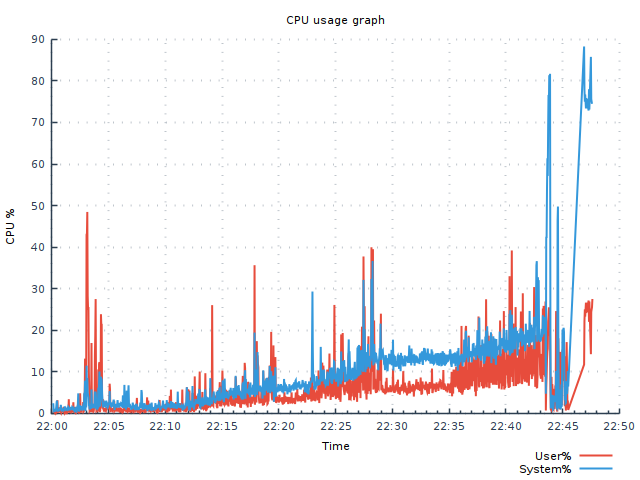
\includegraphics[width=0.95\linewidth]{./context/figures/rpi_cpu.png}
      \caption{CPU usage}
      \label{fig:rpi_cpu}
    \end{subfigure}%
    \begin{subfigure}[b]{.4\textwidth}
      \centering
      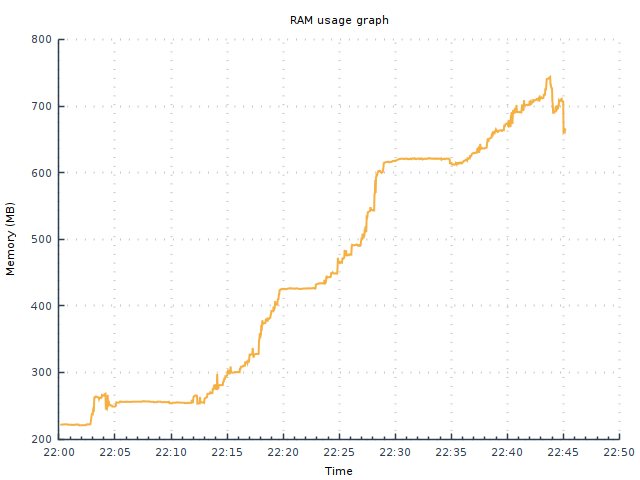
\includegraphics[width=0.95\linewidth]{./context/figures/rpi_ram.png}
      \caption{RAM usage}
      \label{fig:rpi_ram}
    \end{subfigure}
    \centering
    \begin{subfigure}[b]{.4\textwidth}
      \centering
      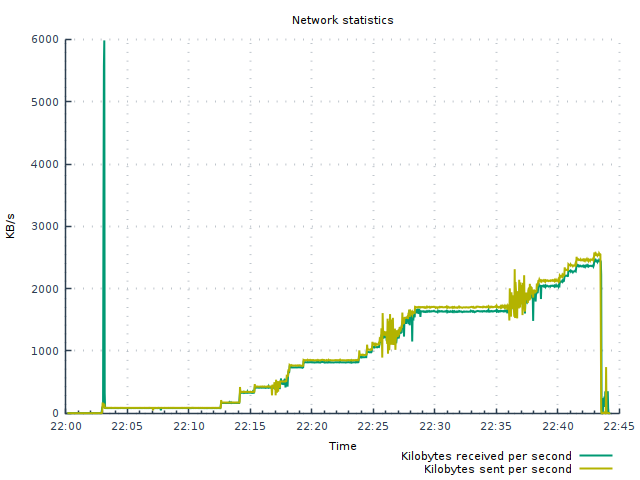
\includegraphics[width=0.95\linewidth]{./context/figures/rpi_netinterface.png}
      \caption{Network throughput}
      \label{fig:rpi_netinterface}
    \end{subfigure}%
  }
  \caption{Performance}
  \label{fig:result_rpi}
\end{figure}

% ------------------------------------------------
\EndChapter
% ------------------------------------------------

% !TeX root = ../../thesis.tex
% ------------------------------------------------
\StartChapter{Experiments and Evaluations}{chapter:experiment}
% ------------------------------------------------

% ------------------------------------------------
\EndChapter
% ------------------------------------------------


% Performance chapter
%\input{./context/performance/performance}

% Conclusion chapter
% !TeX root = ../../thesis.tex
% ------------------------------------------------
\StartChapter{Conclusion}{chapter:conclusion}
% ------------------------------------------------

Write your conclusion here.

% ------------------------------------------------
\EndChapter
% ------------------------------------------------


% Future work chapter
%\input{./context/future-work/future-work}

% ------------------------------------------------

% 參考文獻 References
% !TeX root = ../../thesis.tex
% References and bibliography

% Import the files that contain your references.
% If you set some references file,
% you need to use at least one cite to make Latex work.

\ReferencesFiles{./context/references/paper}{./context/references/misc}{./context/references/book}


% ------------------------------------------------

% 附錄 Appendix
%\input{./context/appendix/appendix}

% ------------------------------------------------
